\documentclass{article}
% Double-blind workshop submission. NOT [final] -- that is the camera-ready
% option and it de-anonymises the author block, which this submission must not.
\usepackage[dblblindworkshop]{neurips_2026}
\workshoptitle{JUDGe (Junior Spotlight Track)}

\usepackage[utf8]{inputenc}
\usepackage[T1]{fontenc}
\usepackage{hyperref}
\usepackage{url}
\usepackage{booktabs}
\usepackage{amsmath}
\usepackage{graphicx}
\usepackage{microtype}
\usepackage{array}

% Title candidates considered:
%   1. "A Deterministic Judge That Cannot See Its Own Evidence"
%   2. "Valid, and Blind: A Grounded Judge That Scores Noise Like Signal"
%   3. "The Correction Loop Erased the Only Signal We Had"
% Selected (1): it states the scope of the failure without implying the judge is
% wrong at what it measures, and without claiming anything is eliminated.
\title{A Deterministic Judge That Cannot See Its Own Evidence}

\author{%
  Anonymous Author(s)\\
  Affiliation\\
  Address\\
  \texttt{email}
}

\begin{document}
\maketitle

\begin{abstract}
We evaluate a deterministic, environment-grounded judge that checks whether an
LLM's explanation cites the sensors a graph explainer actually selected --- no LLM
judges another LLM. On 93 traffic-forecasting scenarios it works exactly as designed,
yet cannot distinguish a real explanation from one whose evidence is a seeded uniform
random draw: precision and hallucination match to four decimals. We trace this to a
near-flat, unstable mask, show a downstream decision agent is equally indifferent,
and report a failed entropy gate. A corrector built to raise grounding erases the one
pre-loop measurement that did separate real evidence from fake.
\end{abstract}

\section{Introduction}

A spatial-temporal graph neural network forecasts speed at a traffic sensor; a
mask-based explainer ranks which other sensors drove that forecast; an LLM turns
the ranking into prose naming locations; a deterministic checker verifies those
locations appear in the ranking. The pipeline is \emph{explainer $\rightarrow$ LLM
$\rightarrow$ verifier $\rightarrow$ decision}. The verifier is a decidable
function of the explanation artifact and a node table, so it is immune by
construction to the position, verbosity and self-enhancement biases afflicting LLM
judges~\citep{zheng2023judging}. That immunity buys less than it appears to. The
judge correctly scores citation--artifact correspondence, cannot tell whether the
artifact carries any information, and a correction loop added to improve grounding
destroys the one signal that would have revealed the evidence was fabricated. Our contribution
is a set of controls --- random and mismatched evidence, a second explainer, a
decision-level replication, a failed detector --- locating which part of a grounded
evaluation stack is load-bearing.

\section{Setup}

The forecaster is a Graph WaveNet-style ST-GNN~\citep{gwnet2019} on METR-LA (207
sensors); the explainer learns a soft node mask after
GNNExplainer~\citep{ying2019gnnexplainer}, and its top-$k$ ($k{=}8$) entries are
rendered into the prompt as the only admissible causes. The judge resolves each
free-text citation to a node-id set via an escalating ladder (exact sensor, exact
region, fuzzy, geographic), counting a hit when that set intersects the top-$k$;
precision, recall, $F_1$ and hallucination $(1-\text{precision})$ follow. The
resolver scores $29/30 = 96.7\%$ on hand-labeled cases --- a \textbf{single-labeler
validation on 30 cases}, not a reliability estimate. Five conditions share one
93-scenario corpus: \textbf{A} (full explanation), \textbf{B} (prediction only),
\textbf{C} (no city context), \textbf{A\_rand} (importances replaced by a seeded
uniform draw) and \textbf{A\_mismatch} (evidence from a different sensor's real
explanation, via a seeded derangement). All use \texttt{llama3.1:8b}; every call is
logged, and all non-LLM stages are seeded and byte-reproducible.

\begin{table}[t]
\centering
\caption{Faithfulness by condition. One 93-scenario corpus, epoch-34 checkpoint,
\texttt{llama3.1:8b}; brackets are 95\% bootstrap CIs (10{,}000 resamples, seed 42).}
\label{tab:main}
\small
\begin{tabular}{lcccc}
\toprule
Condition & Precision & Recall & $F_1$ & Hallucination \\
\midrule
A (full explanation)      & 0.9946 & 0.5927 & 0.7246 [0.6930, 0.7553] & 0.0054 [0.0000, 0.0161] \\
B (no explanation)        & 0.1720 & 0.0712 & 0.0896 & 0.8280 \\
C (no city context)       & 0.9946 & 0.6048 & 0.7277 & 0.0054 \\
A\_rand (random evidence) & 0.9946 & 0.5645 & 0.7013 [0.6681, 0.7334] & 0.0054 [0.0000, 0.0161] \\
A\_mismatch (wrong sensor)& 0.9892 & 0.6008 & 0.7275 [0.6959, 0.7591] & 0.0108 [0.0000, 0.0269] \\
\bottomrule
\end{tabular}
\end{table}

\section{Results}

\paragraph{The judge is valid, and blind.} A\_rand replaces the explainer's
importances with a seeded uniform draw and changes nothing else --- same scenarios,
same predicted speeds, same template, prompt lengths within $0.4\%$ of A. It scores
precision $0.9946$ and hallucination $0.0054$, \emph{identical to A at four decimal
places}, with paired differences of exactly $0.0000$ on both and 95\% CIs
$[-0.0161, +0.0161]$ spanning zero. A\_mismatch, shown a real explanation belonging
to a different sensor, reaches $F_1\ 0.7275$ against A's $0.7246$. Condition B makes
this interpretable: deleting the explanation entirely does collapse the judge
(precision $0.9946 \to 0.1720$, hallucination $0.0054 \to 0.8280$). The judge is not
broken --- it is valid for what it measures, correspondence between citations and a
supplied artifact, and blind to whether that artifact means anything.

\paragraph{The mask is close to flat.} The artifact carried little more information
than noise to begin with. On an independent 207-target sweep of the same explainer,
covering $80\%$ of a target's off-self importance mass takes on average
$146.6\pm4.7$ (congested) and $154.0\pm2.9$ (free-flow) of 206 available
sources.\footnote{Run \texttt{20260824T235016Z\_\_influence\_\allowbreak graph\_solves},
\texttt{metrics.json}.} A ranking
needing three quarters of the network for four fifths of its mass is close to flat,
and the top-8 in every prompt is the head of that flat ranking.

\paragraph{And its top-$k$ is close to unstable.} Flatness predicts instability, and
we measure it three ways. Splitting each target's 24 windows into two stratified
halves and re-deriving the top-8 from each gives a Jaccard of $0.2256$ over the 200
free-flow targets present in both halves and $0.1399$ over the 28 congested ones,
against a two-independent-random-draws reference of $0.0165$ and $0.0182$
respectively --- above chance, but far from a determined object.$^{1}$ Raising the
explainer's sparsity coefficient does not help: over 40 targets the split-half
Jaccard is $0.2323\pm0.1461$ at the committed $\lambda$, $0.2385\pm0.1739$ at
$3\lambda$ and $0.2287\pm0.1831$ at
$10\lambda$.\footnote{Run \texttt{20260825T201433Z\_\_grounding\_without\_information},
\texttt{part4\_metrics.json}, \texttt{settings[]}. Seed-repeat and entropy figures
below come from the same file.} Re-running the explainer at a different random seed
on 10 of those targets recovers only $0.3480$, $0.3149$ and $0.3015$ of the top-8
at the three settings. Even the arithmetic is load-bearing: solving the same target
and window at the same seed on CPU versus MPS agrees on importance \emph{magnitudes}
(Pearson $0.9193$) while agreeing on top-8 \emph{identity} only $0.3991$ of the
time.\footnote{Run \texttt{20260824T235643Z\_\_device\_divergence},
\texttt{device\_divergence.json}; 3 cases, Spearman rank $0.5778$, top-20 Jaccard
$0.3576$.} Substituting a uniform draw for an object this weakly determined is a
smaller intervention than it sounds.

\paragraph{A second explainer scores the same.} On a 28-scenario subset where
SHAP (KernelExplainer) was run beside the mask, the two methods' top-$k$ sets
overlap by a mean Jaccard of $0.0221$ yet receive \emph{identical} judge precision
$0.9821$ and hallucination $0.0179$ ($F_1\ 0.7423$ vs
$0.6918$).\footnote{\texttt{shap\_comparison\_summary.json},
\texttt{aggregate.\{A,D\}} and \texttt{gnn\_vs\_shap\_topk\_overlap}; $n{=}28$.}

\begin{figure}[t]
\centering
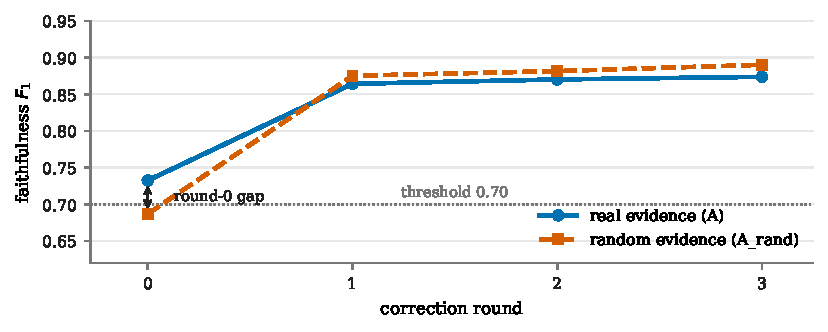
\includegraphics[width=0.76\linewidth]{fig_loop.pdf}
\caption{Faithfulness $F_1$ by correction round, real evidence (A) versus random
evidence (A\_rand), $n{=}93$ each, threshold $0.70$. The arms are separated before
any correction and indistinguishable after one round; by round 3 the fabricated
condition is marginally higher. Series differ in colour, dash and marker so the
figure survives greyscale.}
\label{fig:loop}
\end{figure}

\paragraph{The loop erases the one signal that existed.} One measurement did
separate real from fabricated evidence: before any correction, $64.5\%$ of scenarios
met the $0.70$ grounding threshold on real explanations against $41.9\%$ on random
ones. A corrector --- score the advisory, name the top-$k$ nodes it failed to cite,
re-prompt, up to three rounds --- drives both to the ceiling: real reaches $100.0\%$
at $F_1\ 0.8738$, random $98.9\%$ at $F_1\ 0.8903$, the fabricated condition
finishing marginally \emph{higher} (Figure~\ref{fig:loop}). \textbf{The loop built to
make the system more reliable is precisely what destroys the only measurement that
revealed the evidence was fake.} What survives is agreement between prose and
artifact, which the loop optimises directly; what does not is the diagnostic value
of failing to agree.

\subsection{The blindness reaches the decision, not just the score}

A judge that cannot see its evidence would matter less if a downstream agent could.
We ran the decision simulation on 150 stratified scenarios $\times$ 3 seeds, asking
an agent to choose one of five traffic interventions, scored against a
model-in-the-loop ground truth. Both arms are present for every scenario and seed,
so the contrast is paired \emph{within} scenario and does not involve any baseline.
Showing the agent the real explanation rather than a random one changes accuracy by
$+0.0200$ (95\% CI $[-0.0289, +0.0711]$) and delay reduction by $+0.1153$ mph
(95\% CI $[-1.3158, +1.5452]$), both bootstrapped over 10{,}000 resamples of
scenarios.\footnote{\texttt{paired\_decision\_ab.json} in the grounding run's
processed directory, computed from \texttt{part3\_per\_decision.csv}. Resampling
unit is the scenario, not the decision, because a scenario's three seeds share a
window, a ground-truth action and an explanation.} \textbf{Both intervals span zero.}
At the scenario level the real explanation wins 32 and loses 26 on accuracy with 92
ties, and wins 54 and loses 48 on delay reduction with 48 ties. We deliberately do
not frame this against the no-explanation baseline: that baseline is unstable across
sample sizes --- $0.2756$ accuracy on this 150-scenario subset against $0.2327$ on
the full 444 --- by more than either explanation arm exceeds it on either, so an
above-baseline test would report the sampling, not the effect.

\subsection{A cheap detector that did not replicate}

If the top-$k$ is unstable because the mask is flat, then mask entropy should
predict instability, and entropy is computable from a single solve whereas measuring
stability costs a second one. We pre-registered that test before running it:
normalised Shannon entropy of the off-self mask, correlated against the same
split-half top-8 Jaccard, with success defined in advance as Spearman
$\rho < -0.30$ \emph{and} a bootstrap CI excluding zero, plus a threshold chosen on
the sweep alone flagging all 12 committed explanations. Pooled over 120
(target, setting) pairs, $\rho = -0.2008$ with 95\% CI $[-0.4229, +0.0452]$ for the
entropy of the window-averaged mask and $\rho = -0.1732$, CI $[-0.3938, +0.0513]$
for the mean per-window entropy --- the second being the only form obtainable from a
single solve, and therefore the only one that would have made this cheap. Both
intervals include zero; the threshold flagged $3$ of $11$ distinct committed
explanations, not all of
them.\footnote{\texttt{verdicts.json}, \texttt{P4}; both sub-verdicts recorded
FALSIFIED. The 12 committed explanation files cover 11 distinct (target, window)
pairs.} \textbf{Both pre-registered criteria are falsified and we report them as
such.} A single-setting version of this test at $n{=}40$ did appear to pass; it did
not survive the full pool, which is the ordinary fate of an underpowered result and
the reason the criteria were fixed in advance.

\section{Facet mapping}

A deterministic checker's coverage of judge-quality facets is unusually easy to
state, because most of it is settled by construction rather than by measurement.
\emph{Surface-form sensitivity}, \emph{positional bias}, \emph{sycophancy} and
\emph{inter-judge inconsistency} are all removed outright: there is no judge model
to exhibit them, the same input yields the same verdict on every run, and rerunning
the scorer changes nothing. \emph{Verbosity bias} is likewise absent: the score
depends on the citation array, not answer length. Against that, three facets are
untouched. \emph{Criteria drift} is not addressed at
all: the evaluation field is self-declared by the same project that built the system
being evaluated, with no external specification and no community standard.
\emph{Reasoning-chain validity} is not addressed: the judge checks which locations
are cited, never whether the causal story told about them is coherent or correct,
so a reversed edge or an invented propagation order scores clean. And \emph{construct validity} is exactly what this paper puts in
question: a judge scoring random evidence identically to real evidence is measuring
citation compliance, not grounding.
A filled disclosure template is provided in Appendix~\ref{app:disclosure}.

\section{Limitations}

\textbf{(a)} Faithfulness here is agreement with what the model was \emph{shown},
not with what is \emph{true}; there is no ground-truth causal attribution for a real
road network, which is why A\_rand is diagnostic at all. \textbf{(b)} Condition B
differs from A in several ways at once (no importance table, no propagation path,
different retrieved context), so we make no mechanistic claim about which absence
causes its collapse. \textbf{(c)} One claim type (citation membership), a
self-declared evaluation field, and a single LLM family per run: every condition in
Table~\ref{tab:main} used \texttt{llama3.1:8b}, and we make no cross-model claim ---
a second model appears only in a separate cross-city study that is excluded here as
a different corpus. \textbf{(d)} Conditions A/B/C and A\_rand/A\_mismatch were
scored by different versions of the entity resolver (fixed 2026-07-21, between
runs). This does not affect the precision/hallucination results above --- precision
is identical to four decimal places between A and A\_rand --- since a
resolver-version change can only affect which citations are matched, not whether a
match is correct. It may affect the smaller recall/$F_1$ differences between
conditions; a same-corpus proxy bounds the resolver's own contribution at
approximately 0.005--0.014 $F_1$. We restrict our central claim to the
precision/hallucination axis, which is unaffected. \textbf{(e)} The resolver was
validated on 30 hand-labeled cases by a \emph{single labeler}; there is no second
annotator and no inter-annotator agreement, so $96.7\%$ is a development check, not
a measured reliability. \textbf{(f)} The supporting measurements carry small
samples of their own: the seed-repeat Jaccard rests on 10 targets, the device
comparison on 3 cases, the SHAP comparison on 28 scenarios, and the congested
split-half on 28 targets. We report them as indicative, and none of them carries the
central claim, which rests on Table~\ref{tab:main}. \textbf{(g)} The decision
simulation's ground truth is model-in-the-loop --- what the trained forecaster
believes an intervention would do, not an observed outcome --- so it inherits that
model's biases and is internally consistent rather than externally valid.

\section{Related work}

LLM-as-judge biases are set out by~\citet{zheng2023judging}.
Citation and attribution evaluation are formalised by ALCE~\citep{gao2023alce} and
AIS~\citep{rashkin2023ais}, which separates attribution from correctness by
definition; our results instantiate that separation where no gold reference exists.
\citet{shi2023distracted} show irrelevant context degrades task accuracy --- here the
irrelevant content is the evidence the model is told to cite, and the measured
quantity is compliance.

The stability results sit on an existing line of work on GNN-explainer evaluation.
\citet{sanchez2020evaluating} benchmark attribution against computable ground truth
on synthetic graphs; our setting has none, which is what makes a randomised-evidence
control necessary rather than optional. \citet{faber2021ground} show that comparing
explanations to ground truth is itself unsound when the GNN does not use the
ground-truth edges, separating responsible, causing and explanatory motifs; our
mismatch is one step further downstream, between an explanation and a judge that
consumes it. \citet{agarwal2023evaluating} provide generators and a library for
evaluating explanation quality. Our numbers agree with that literature; what we add
is the downstream consequence --- an unstable, near-flat attribution is
indistinguishable from noise to the verifier and to the agent built on it.

To our knowledge this is the first evaluation where the cited source is a
\emph{GNN-explanation artifact}, checked by a \emph{deterministic} verifier with no
gold reference, paired with a \emph{correction loop} whose effect on the noise
signal is measured.\footnote{C\_RICH (fuller context) and D\_CONTRA (contradictory context) ran on
this corpus in a separate LLM draw and did not move hallucination materially; being
a different draw they are omitted from Table~\ref{tab:main}.}

\begin{thebibliography}{9}
\bibitem[Agarwal et al.(2023)]{agarwal2023evaluating}
C.~Agarwal, O.~Queen, H.~Lakkaraju, and M.~Zitnik.
\newblock Evaluating explainability for graph neural networks.
\newblock \emph{Scientific Data}, 10:144, 2023.

\bibitem[Faber et al.(2021)]{faber2021ground}
L.~Faber, A.~K.~Moghaddam, and R.~Wattenhofer.
\newblock When comparing to ground truth is wrong: On evaluating GNN explanation
methods.
\newblock In \emph{KDD}, 2021.

\bibitem[Gao et al.(2023)]{gao2023alce}
T.~Gao, H.~Yen, J.~Yu, and D.~Chen.
\newblock Enabling large language models to generate text with citations.
\newblock In \emph{EMNLP}, 2023. arXiv:2305.14627.

\bibitem[Rashkin et al.(2023)]{rashkin2023ais}
H.~Rashkin, V.~Nikolaev, M.~Lamm, L.~Aroyo, M.~Collins, D.~Das, S.~Petrov,
G.~S.~Tomar, I.~Turc, and D.~Reitter.
\newblock Measuring attribution in natural language generation models.
\newblock \emph{Computational Linguistics}, 49(4):777--840, 2023.

\bibitem[Sanchez-Lengeling et al.(2020)]{sanchez2020evaluating}
B.~Sanchez-Lengeling, J.~N.~Wei, B.~K.~Lee, E.~Reif, P.~Wang, W.~W.~Qian,
K.~McCloskey, L.~J.~Colwell, and A.~B.~Wiltschko.
\newblock Evaluating attribution for graph neural networks.
\newblock In \emph{NeurIPS}, 2020.

\bibitem[Shi et al.(2023)]{shi2023distracted}
F.~Shi, X.~Chen, K.~Misra, N.~Scales, D.~Dohan, E.~H.~Chi, N.~Sch\"arli, and
D.~Zhou.
\newblock Large language models can be easily distracted by irrelevant context.
\newblock In \emph{ICML}, 2023. arXiv:2302.00093.

\bibitem[Wu et al.(2019)]{gwnet2019}
Z.~Wu, S.~Pan, G.~Long, J.~Jiang, and C.~Zhang.
\newblock Graph WaveNet for deep spatial-temporal graph modeling.
\newblock In \emph{IJCAI}, pages 1907--1913, 2019.

\bibitem[Ying et al.(2019)]{ying2019gnnexplainer}
R.~Ying, D.~Bourgeois, J.~You, M.~Zitnik, and J.~Leskovec.
\newblock GNNExplainer: Generating explanations for graph neural networks.
\newblock In \emph{NeurIPS}, 2019. arXiv:1903.03894.

\bibitem[Zheng et al.(2023)]{zheng2023judging}
L.~Zheng, W.-L. Chiang, Y.~Sheng, S.~Zhuang, Z.~Wu, Y.~Zhuang, Z.~Lin, Z.~Li,
D.~Li, E.~P.~Xing, H.~Zhang, J.~E.~Gonzalez, and I.~Stoica.
\newblock Judging LLM-as-a-judge with MT-Bench and Chatbot Arena.
\newblock In \emph{NeurIPS Datasets and Benchmarks}, 2023. arXiv:2306.05685.
\end{thebibliography}

\appendix

\section{JUDGe Judge Deployment Disclosure Template (filled)}
\label{app:disclosure}

\textbf{Judge identity.} Deterministic program, not a model. Entity resolver plus
set-intersection scoring over the explainer's top-$k$. No LLM is used to judge
another LLM's output. Version-sensitive: the resolver was changed 2026-07-21.

\textbf{What is judged.} A single claim type: whether a free-text location in the
LLM's \texttt{cited\_causes[]} array resolves to a node set intersecting the
explainer's top-$k$. The LLM's prose is not read. A refusal (no citations) scores
hallucination $1.0$, identical to confidently inventing causes.

\textbf{Scale and outputs.} Precision, recall, $F_1$, hallucination rate
$(1-\text{precision})$, per advisory, averaged over 93 scenarios.

\textbf{Ground truth.} None available. The reference is the explainer's own
top-$k$, so the judge measures correspondence, not correctness.

\textbf{Validation.} Resolver: $29/30 = 96.7\%$ on hand-labeled cases, one
labeler, no inter-annotator agreement, threshold set at $90\%$ in advance.

\textbf{Known blind spots.} Cannot distinguish real from random evidence
(Table~\ref{tab:main}); cannot distinguish overreach from falsehood, since both
score as $1-\text{precision}$; does not read the reasoning chain; scores a
refusal identically to a fabrication.

\textbf{Criteria provenance.} Self-declared by the authors of the system being
evaluated. Not externally specified, not community-standardised.

\textbf{Reproducibility.} All non-LLM stages seeded and byte-reproducible. LLM
calls are logged in full but are \emph{not} byte-reproducible: they run at
temperature $0.1$ on an unseeded sampling path, chosen so results remain
comparable with previously committed numbers produced on that path.

\section{Claim-to-source map}
\label{app:sources}

Every number in the main text traces to one of the following. Run directories are
under \texttt{evaluation/results/}; \texttt{GWI} abbreviates run
\texttt{20260825T201433Z\_\_grounding\_without\_information}.

\footnotesize
\begin{tabular}{@{}>{\raggedright\arraybackslash}p{0.34\linewidth}>{\raggedright\arraybackslash}p{0.24\linewidth}>{\raggedright\arraybackslash}p{0.36\linewidth}@{}}
\toprule
Claim & Value & Source \\
\midrule
A / B / C rows & Table~\ref{tab:main} & \texttt{claims.csv} $\leftarrow$ \texttt{faithfulness\_summary.json} \\
A\_rand / A\_mismatch rows & Table~\ref{tab:main} & \texttt{claims.csv} $\leftarrow$ GWI \texttt{part1\_summary.json} \\
Bootstrap CIs, paired diffs & 10k, seed 42 & GWI \texttt{part1\_summary.json}, \texttt{bootstrap\_ci} \\
Corpus, epoch 34, $n{=}93$ & 2026-07-05/06 & \texttt{claims\_provenance.json}, \texttt{corpus} \\
Prompt lengths within 0.4\% & +0.18\%, +0.38\% & GWI \texttt{part1\_token\_parity.json} \\
80\% mass of importance & 146.6$\pm$4.7 / 154.0$\pm$2.9 of 206 & \texttt{20260824T235016Z\_\_\allowbreak influence\_\allowbreak graph\_\allowbreak solves}, \texttt{metrics.json} \\
Split-half Jaccard, 207-target & 0.2256 / 0.1399; ref 0.0165 / 0.0182 & same file, \texttt{per\_regime.*.stability} \\
Split-half Jaccard, 3 $\lambda$ & 0.2323 / 0.2385 / 0.2287 & GWI \texttt{part4\_metrics.json}, \texttt{settings[]} \\
Seed-repeat Jaccard, 3 $\lambda$ & 0.3480 / 0.3149 / 0.3015 ($n{=}10$) & same file \\
CPU vs MPS divergence & Pearson 0.9193, top-8 J 0.3991 & \texttt{20260824T235643Z\_\_\allowbreak device\_\allowbreak divergence}, \texttt{device\_\allowbreak divergence.json} \\
SHAP overlap and scores & J 0.0221; $F_1$ 0.7423 / 0.6918 & \texttt{shap\_comparison\_summary.json} \\
Round-0 grounding & 64.5\% real / 41.9\% random & \texttt{active\_\allowbreak grounding\_\allowbreak summary.json}; GWI \texttt{part2\_summary.json} \\
Loop curve, Figure~\ref{fig:loop} & real $F_1$ 0.7323$\to$0.8738; random 0.6868$\to$0.8903 & same two files, \texttt{per\_round[]} \\
Loop reach endpoints & 100.0\% / 98.9\% & same two files \\
Paired decision contrast & $+0.0200$; $+0.1153$ mph & GWI \texttt{paired\_decision\_ab.json} \\
Baseline instability & 0.2756 ($n{=}150$) vs 0.2327 ($n{=}444$) & same file, \texttt{raw\_baseline\_instability} \\
Entropy gate $\rho$ and CIs & $-0.2008$, $-0.1732$; 3/11 flagged & GWI \texttt{verdicts.json}, \texttt{P4} \\
Resolver 29/30 = 96.7\% & threshold 0.90 & \texttt{resolver\_accuracy.json} \\
Resolver proxy 0.005--0.014 $F_1$ & same-corpus bound & \texttt{claims\_provenance.json} \\
\bottomrule
\end{tabular}
\normalsize

\end{document}
